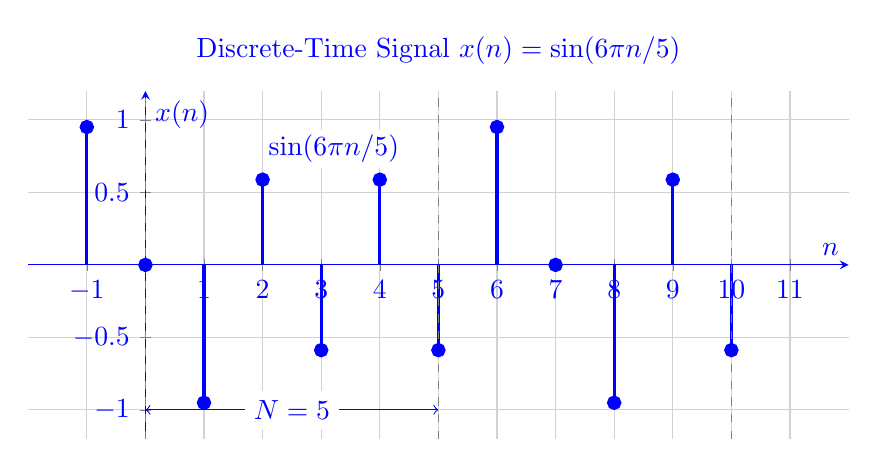
\begin{tikzpicture}
\begin{axis}[
    width=12cm,
    height=6cm,
    axis lines=middle,
    xlabel={$n$},
    ylabel={$x(n)$},
    title={Discrete-Time Signal $x(n) = \sin(6\pi n/5)$},
    xmin=-2, xmax=12,
    ymin=-1.2, ymax=1.2,
    xtick={-1, 0, 1, 2, 3, 4, 5, 6, 7, 8, 9, 10, 11},
    ytick={-1, -0.5, 0, 0.5, 1},
    grid=both,
    grid style={gray!15},
    major grid style={gray!35},
    ycomb, % Discrete-time plot
    mark=*, mark size=2pt, blue,
]

% Plot the discrete-time sinusoidal signal
\addplot[ycomb, blue, very thick, mark=*, mark size=2pt] coordinates {
    (-1, 0.951) (0, 0) (1, -0.951) (2, 0.588) (3, -0.588) (4, 0.588) (5, -0.588) (6, 0.951) (7, 0) (8, -0.951) (9, 0.588) (10, -0.588)
};

% Add period markers
\draw[dashed, gray] (0, -1.2) -- (0, 1.2);
\draw[dashed, gray] (5, -1.2) -- (5, 1.2);
\draw[dashed, gray] (10, -1.2) -- (10, 1.2);

% Add period label
\draw[<->] (0, -1) -- (5, -1) node[midway, fill=white] {$N = 5$};

% Add annotation
\node[anchor=west, fill=white, inner sep=2pt] at (2, 0.8) {$\sin(6\pi n/5)$};

\end{axis}
\end{tikzpicture}
